\chapter{Background}
\label{cha:background}
This chapter provides an overview of the text mining field along with previous work in the area and all necessary background information required to understand the major tasks involved in this project.

\section{Text Mining}
\label{sec:textmining}
The information available in the world is growing exponentially, and the majority of this information(widely estimated at roughly 80\%) is unstructured. This is where text mining comes in, also referred to as Knowledge Discovery from Text(KDT).
``Text mining is the process of extracting interesting information and knowledge from unstructured text''\cite{hotho-etal-ldv-2005} and its applications tend to work in two steps, first using an Information Retrieval(IR) application to narrow the search space, and then they extract significant parts of the retrieved texts\cite{Polajnar2006}. This general process usually involves structuring a source text by means of parsing and other linguistic analysis, then finding patterns in this structured data and then interpreting this output.

Text mining is fundamentally different from standard web searching in that web searches rely primarily on information that is already known. However, the goal of text mining is to discover interesting, previously unknown information\cite{Gupta_Lehal_2009}.
There is however one key issue introduced by text mining; natural language is used by humans for communication and recording information, while computers are incapable of interpreting natural language. Humans are naturally able to find linguistic patterns in text and understand the semantics of what is being said. Computers, on the other hand, face difficulties in interpreting variations in written text through spelling, colloquialism and also the general context of the text. Nonetheless, computers have what humans do not, that is, computers are much more capable of processing large datasets at very high speeds, particularly in comparison to the human being. Thus, the objective of text mining is to combine the best of these both by creating an application that can retrieve relevant documents and then apply linguistic patterns which may be rule-based, using human-defined rules, or taught by means of machine learning techniques. This project takes the rule-based approach and as such only these techniques will be discussed.

An example of the text mining process can be seen in Figure~\ref{fig:tm}.
\begin{figure}[t]
\begin{center}
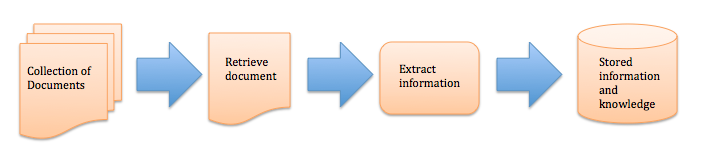
\includegraphics[width=15cm]{tm}
\end{center}
\caption{The text mining process\cite{Gupta_Lehal_2009}}
\label{fig:tm}
\end{figure}

\subsection[Information Retrieval]{Information Retrieval(IR)}
IR is the process of retrieving textual documents which may contain the answers to questions but do not answer these themselves\cite{hotho-etal-ldv-2005}. Information retrieval is fundamentally a web search working off user queries representing an information need. The process works by searching a collection of documents, and then retrieving those matching a user query depending on relevance. The approach to calculating relevance is dependent upon the actual IR engine itself, generally working on the frequency of specific key terms in each of these documents, and usually assigns a relevance rank to each document. This allows a sorting amongst the results and gives improved results, especially when given a limited number of results.

The IR tasks in this project will mainly be carried out on Twitter's systems, and as such, besides the core concept of IR, its internal specifics are not in the scope of this report.

\subsection[Natural Language Processing]{Natural Language Processing(NLP)}
NLP, in the scope of this project, is the process of extracting information from natural language\cite{Healey98}, that is, any language written or spoken by humans. This involves parsing and processing unstructured text to be able to gain meaningful knowledge from it. Nowadays most natural language processing is done using machine learning techniques, however, in the past implementations were based on large sets of coded `rules'. These rules are used to define certain linguistic features in the text in order to understand the semantics behind it. NLP is a major field of research at present and also has applications in both information retrieval and information extraction.

There are many methods involved in NLP tasks and some of these will now be further explored.

\subsubsection{Tokenisation}
Tokenisation is the process of splitting a stream of text into singular words or phrases, otherwise known as tokens. These tokens usually form the basis of further NLP work. While it can be a straightforward process when using Standard English, the definition of a word, from the tokeniser's point of view, can be somewhat ambiguous. This is particularly true when considering the use of apostraphes. Figure~\ref{fig:tokenisation} shows an example of the different ways of tokenising the word \emph{don't}.

\begin{figure}[h!]
  \centering
  \setlength{\unitlength}{0.0125in}
\begin{picture}(80,105)( -20, 0)
\thicklines
\put(0,100){\framebox{don't}}

\put(0,80){\framebox{dont}}

\put(0,60){\framebox{don}}
\put(30,60){\framebox{'t}}

\put(0,40){\framebox{don}}
\put(30,40){\framebox{t}}

\put(0,20){\framebox{do}}
\put(25,20){\framebox{n't}}

\put(0,0){\framebox{do}}
\put(25,0){\framebox{nt}}
\end{picture}

  \caption{The different ways of tokenising the word \emph{don't}
    \label{fig:tokenisation}}
\end{figure}

These variations can be problematic in terms of the results being output for certain user queries. For example, in the case of these differing tokenisations of \emph{don't}, a user search for the word \emph{don} would return true twice, but should be false in the actual context. The importance of normalisations is highlighted tokenising tweets because a lot of users do not use apostrophes, either due to ease when typing, or in order to reduce the number of characters being used. Thus, varying spellings of the terms should not be tokenised differently.

\subsubsection{Normalisation}
Once text has been tokenised, these words may need normalising. Normalisation accounts for the several variations in spelling. For example, if you want to search for \emph{Mozilla~Firefox} you would want an IR engine to return not only documents containing the exact query but also those containing terms such as \emph{Firefox}, \emph{firefox} or \emph{mozilla~firefox}. Not doing this would obviously yield fewer results, or in the case of information extraction, it may suggest that \emph{Mozilla~Firefox} and \emph{mozilla~firefox} are two different things. Thus, normalisation is required to successfully map equivalent classes of terms.

\subsubsection{Stop Words}
Stop words are very commonly used words like \emph{a}, \emph{and} or \emph{the}. By creating a list of these terms, a \emph{stop list}, a natural language parser can remove these terms from the source text as they hold little or no value in matching queries to documents. In modern systems, however, stop lists are not widely used as they provide little gain in terms of efficiency\cite{manning2008}.

\subsubsection{Part of Speech(POS) Tagging}

\subsubsection{Stemming and Lemmatisation}


\subsection[Information Extraction]{Information Extraction(IE)}

\subsubsection{Named Entity Recognition(NER)}

\section[Sentiment Analysis]{Sentiment Analysis and Opinion Mining}

\section{Twitter Mining}
There has been several previous works on text mining Twitter posts, however, the bulk of these have focussed primarily on biomedicine and the financial sector.


% MOVE TWITTER API HERE? FROM IMPLEMENTATION CHAPTER
